%Instruct LaTeX that you would like to format an article and are using a4paper, default is US Letter size!
\documentclass{article}

%Set up a4paper size and sensible margins
\usepackage[a4paper, tmargin=2cm, bmargin=2cm, hscale=0.75]{geometry}
\usepackage[cm]{fullpage}
\usepackage{listings}
\usepackage[font=small]{caption}
%Include support for graphics! 
\usepackage{graphicx}
%Include support for url linking
\usepackage[hidelinks]{hyperref}
\usepackage{amsmath}
\usepackage{wrapfig}


\title{Applications of Optical Ray Tracer to Lens Optimisation and Rainbow Formation Analysis}
\author{ Stefanos Mousafeiris - 00951054 }
\date{\today}

\begin{document}

\maketitle


\begin{abstract}
An optical ray tracer was built using Python and used to model and examine optical systems such as a biconvex lens and a raindrop. Applications of these models to lens optimisation through the minimisation of spherical aberrations and rainbow formation analysis were investigated, and results included the approximate optimal ratio of lens curvatures of $10:3$, and the angular widths of the primary rainbow, secondary rainbow, and Alexander's dark band, which were found to be $1.6^{\circ}$, $3^{\circ}$, and $8.2^{\circ}$ respectively.
\end{abstract}


\section{Introduction}
Optical ray tracing is a method of solving problems in optics by representing light waves as infinitely narrow rays and propagating them through various optical elements and media. Using rays is a valid approximation as long as the size of anything the light waves interact with is much larger in comparison to the light's wavelength.

This method allows for the modelling of optical systems and their properties, which can then be examined in more detail. In this investigation, an optical ray tracer was programmed and the propagation of light through various optical systems was simulated to examine the behaviour of said systems. The investigation is separated into two parts: the optimisation of the curvatures of a biconvex lens with respect to the RMS spread of light at the desired focal point for a given thickness and refractive index, and the analysis of the physics behind rainbow formation in raindrops.

\section{Experimental Method}
A model of all the optical elements that were required to simulate the optical systems of interest was first built using an object oriented approach in Python 2.7, along with a model for the useful geometrical arrangements of light rays. 

The first use of that model was to optimise a biconvex lens of given thickness and refractive index for the desired focal length by changing the curvatures of the two sides of the lens. In this case, the optimisation refers to the minimisation of the root mean square (RMS) spread of a light beam at the focal point. The beam consisted of an arrangement of rays, and the RMS spread was calculated as the RMS of the distances of the individual rays from the focal point on a plane parallel to the lens at the focal length.

The optimisation of the curvatures was done by initially minimising the RMS spread within the bounds dictated by the Lensmaker Equation for thick lenses, i.e. the Gullstrand Equation\cite{lensmaker}, using one of the two curvatures as the variable argument and the RMS spread as the optimisation metric. The Gullstrand equation is:
\begin{equation}\label{eq:lensmaker}
\frac{1}{f} = (n-1)(C_1 - C_2 + \frac{(n-1)d}{n} C_1 C_2)
\end{equation}
where $C_1,C_2$ are the curvatures, $n$ is the refractive index, $d$ is the lens thickness, and $f$ is the focal length. The resulting curvatures from the first bounded, one-dimensional optimisation were then used as the initial guess for a second, unbounded, two-dimensional optimisation of the RMS, where both curvatures were variable arguments. This optimisation was then reiterated for a range of focal lengths. 

To investigate the physics of rainbow formation, a raindrop optical element was modelled, and rays of different wavelengths were propagated through that raindrop to simulate rainbow formation due to white light dispersion in water. Intensity of light was modelled as the number of white light rays sent into the raindrop, so that reflectance and transmittance could be probabilistically simulated by using the percentage of the intensity reflected or transmitted as a probability instead. These probabilites were calculated using the Fresnel equations\cite{fresnel}. In the limit of high intensity, this probabilistic approach should correspond to the actual physics.

By sending white light rays parallel to the ground into the raindrop, the angle and intensity at which each propagated ray is seen by an observer on the ground were measured and plotted with respect to the initial height of the ray relative to the raindrop, called impact parameter\cite{impact}. The results were then used to explain some key properties of rainbows, such as the origin of the secondary rainbow and Alexander's dark band.



\section{Results}
\subsection{Lens Optimisation}

\begin{wrapfigure}{r}{0.45\textwidth}
\centering
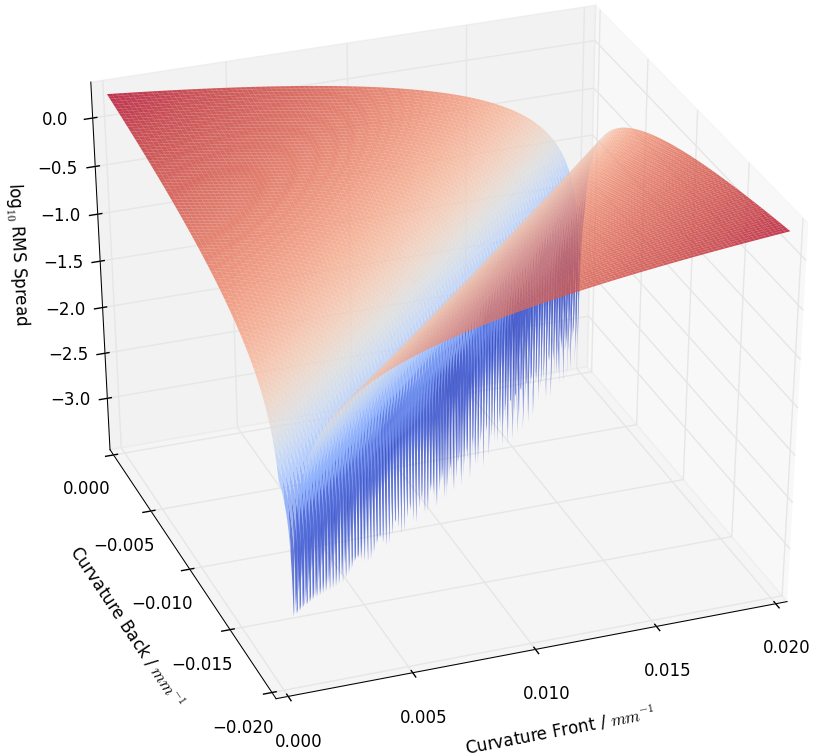
\includegraphics[width=0.45\textwidth]{surface_plot}
\caption{Surface plot of $\log_{10}$RMS spread with respect to lens curvatures.}
\label{fig:surface}
\end{wrapfigure}

For any set of given specifications, i.e. lens thickness and refractive index, there should be a pair of curvatures of the lens that will yield the optimal RMS spread at the focal point. Ideally, the optimal spread should be lower than the diffraction limit of the light beam being focused, so that the rays that make up the focal point are indistinguishable.

In this investigation, a lens of thickness $5\,mm$ and refractive index $n=1.5168$ was modelled for a light beam of wavelength $588\, nm$ and diameter $10\,mm$. Figure \ref{fig:surface} illustrates how the logarithm of the RMS spread varies with the two curvatures of the lens. The sharp negative peaks are not representative of the actual behaviour of the spread, but are a limitation of the numerical approach used to produce the data. However, there is a clear path on the surface plot that minimises the spread, as only few of the curvature combinations yield a focal length close to the desired one. The path is almost entirely governed by equation \ref{eq:lensmaker}, which was used to get an initial estimate of the optimal curvatures on the minimum spread path, and consequently to get the optimal curvatures.

\begin{wrapfigure}{l}{0.49\textwidth}
\centering
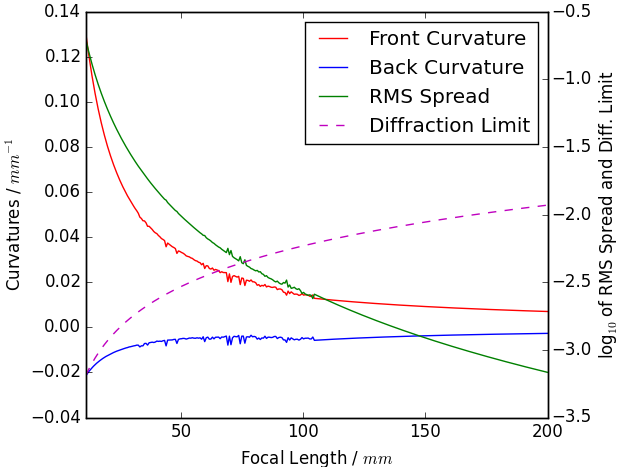
\includegraphics[width=0.49\textwidth]{curvatures_vs_focal_length_7_10}
\caption{Plot of optimal curvatures and their respective RMS spread and diffraction limit against focal length.}
\label{fig:curvatures}
\end{wrapfigure}

This process was iterated over a range of focal lengths to investigate the behaviour of the curvatures, but also to evaluate how the optimal RMS spread compares to the diffraction limit over the same range of focal lengths. Figure \ref{fig:curvatures} illustrates the behaviours of the aforementioned quantities.

A clear trend is that the curvatures of the lens both tend asymptotically towards zero, one from the positive side and one from the negative. This means that for larger focal lengths, the optimal lens will tend to be flatter, which is reasonable as the rays will need to be refracted by a smaller angle. More notably, the magnitude of the curvature of the front lens seems to be consistently larger than the magnitude of the curvature of the back of the lens, and at larger focal lengths $>100\,mm$ their ratio is approximately $10:3$. It was calculated to be $\approx 3.13$ with negligible uncertainty. This is a non-trivial result, as it implies that for any singlet converging lens, there is an orientation that results in less aberrations than the other and thus a lower RMS spread. The correct orientation is thus the one where the front of the lens, where the light is incident, has the larger curvature. Combining these two results, it can also be inferred that in the limit of high focal lengths, the optimal lens would be a plano-convex lens with the convex side in the front. This would be the case for telescopes, as the incoming light is approximately collimated, and the focal length is approximately infinity.

From figure \ref{fig:curvatures}, it is also clear that the optimal RMS spread at the focal point decreases with focal length, while the diffraction limit increases. This was also expected, as for larger focal lengths the diameter of the diffracted beam becomes infinitesimal in comparison, and can thus be approximated as a ray, which has no spread. The diffraction limit increasing is reasonable, as the farther away the focal length is, the harder it is to resolve the projection. An interesting focal length is $\approx75\,mm$, at which, as it can be seen from figure \ref{fig:curvatures}, the spread crosses the diffraction limit. Beyond that critical length, the rays cannot be distinguished from one another at the focal point, and the optical setup can be classified as a diffraction-limited system, i.e. limited only by its theoretical diffraction limit. For focal lengths smaller than the critical length, the rays are distinguishable and are thus not optimally focused. Therefore, the larger the diameter of the refracted beam, the farther away the focal length needs to be to operate at the diffraction limit, which is a reasonable result. The spikes in figure \ref{fig:curvatures} are due to the limitations of the numerical approach.


\subsection{Rainbow Formation}
For the sake of convenience, the results in this section are coloured depending on the wavelength of the analysed rays. The simulated white light used consisted of a range of wavelengths from $390\,nm$ to $700\,nm$, the dispersion was modelled according to an empirical expression\cite{dispersion}, and the raindrop was modelled as a sphere, which is a reasonable approximation for diameters smaller than $2\,mm$\cite{raindrop}. Figure \ref{fig:raindrop} illustrates the way rainbow formation works. White light is sent at a height relative to the raindrop's centre, called impact parameter, which then propagates through it by either reflecting or refracting. Because of dispersion and reflectance, a part of the refracted white light will form a rainbow observable from the ground at a specific range of angles. A secondary rainbow is formed by white light coming from below the droplet's centre height.

\begin{figure}[h]
  \begin{minipage}[b]{0.55\textwidth}
	\centering
   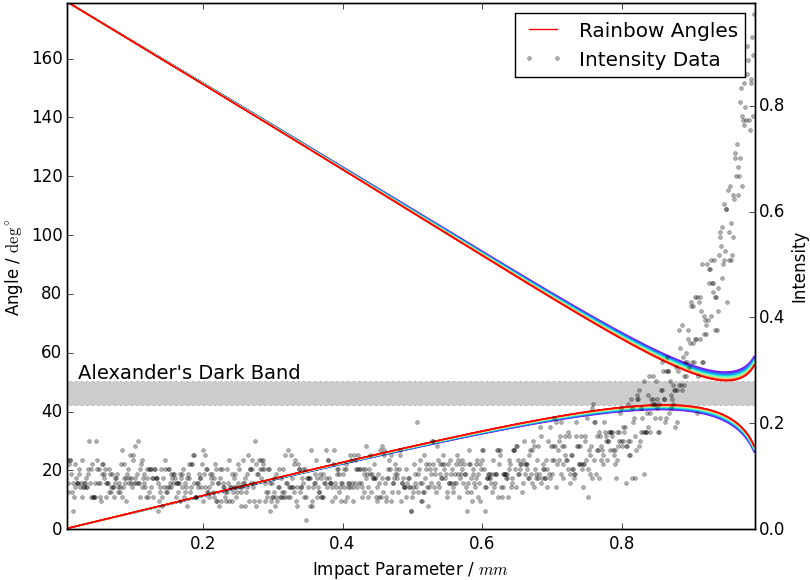
\includegraphics[width=\textwidth]{rainbow}
   \caption{Plot of observation angle of component wavelengths of rainbow and of intensity with respect to the impact parameter.}
	\label{fig:rainbow}
  \end{minipage}
  \begin{minipage}[b]{0.5\textwidth}
	\centering
   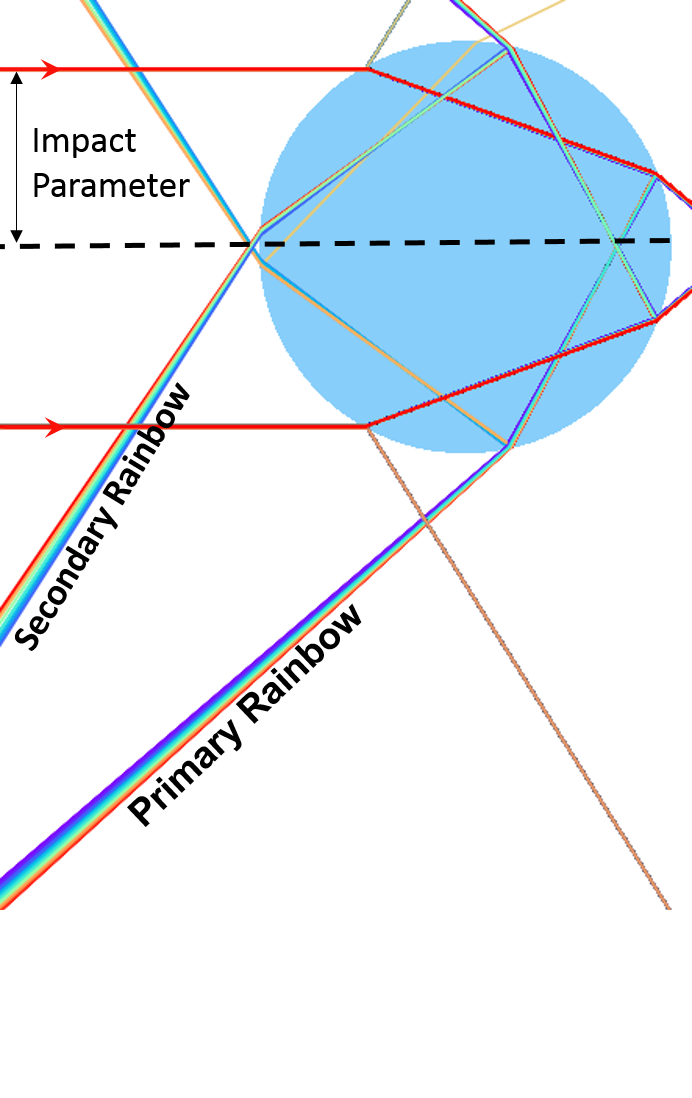
\includegraphics[width=0.5\textwidth]{rainbowdrop}
   \caption{Diagram of white light scattering in raindrop.}
	\label{fig:raindrop}
  \end{minipage}
\end{figure}

By simulating white light falling in the raindrop for the entire range of possible values of the impact parameter, i.e. from 0 to the raindrop's radius both below and above its centre's height, the angles at which light of each wavelength was observed from the ground were measured and plotted against the impact parameter in figure \ref{fig:rainbow} along with the intensity of the received light. The impact parameter was taken to be positive for both directions relative to the raindrop's centre.

From figure \ref{fig:rainbow}, the primary rainbow, at its highest intensity and clarity of distinct colors, spans an angular width of approximately $1.6$ degrees, from $40.7^{\circ}$ to $42.3^{\circ}$, and the secondary rainbow spans a width of approximately $3$ degrees, from $50.5^{\circ}$ to $53.5^{\circ}$. For angles below and above those ranges, light can still be observed, but the angular separation between the rays of different wavelengths is small and the intensity low, essentially making it dim white light. One of the most notable results is that for the range of angles between the two rainbows, namely $42.3^{\circ}$ to $50.5^{\circ}$, there is no light contribution from low-class rays, i.e. reflected inside raindrop less than 3 times. This is known as Alexander's dark band, and can be observed in the cases where a secondary rainbow is present as a dark arch between the two rainbows. Its existence can be then attributed to the geometry of ray propagation within a sphere.

The intensity pattern, plotted with arbitrary units, is flat for most of the range of the impact parameter, and peaks at the upper end. This means that almost all of the contribution to the rainbow intensity is from light falling near the top and bottom edges of the raindrop, which is an expected consequence of Fresnel's equations for reflectance.

\pagebreak
\section{Conclusion}
The aim of this investigation was to build an optical ray tracer using Python and use it to model and examine optical systems. Its applications that were explored were the lens optimisation through minimisation of aberrations via the use of the RMS spread of a light beam at the focal point as an optimisation metric, and the analysis of the optics behind rainbow formation through the use of a probabilistic model of Fresnel reflectance.

Some notable results from the lens optimisation were the asymptotic behaviour of the optimal curvatures of a lens with respect to the focal length, and the semi-constant ratio of said curvatures of approximately $10:3$. The most important inference made from these results was that at the limit of the focal length going to infinity, the most effective lens would be plano-convex with its curved surface facing the incident light, which is indeed the case for telescopes. Other results in the optimisation include the existence of a critical focal length, at which, for a lens of given thickness and refractive index, the RMS spread of the focused beam becomes comparable to the diffraction scale of the system. A possible extension of this project could be to explore the behaviour of this critical focal length for a varying lens thickness and refractive index.


The rainbow formation analysis also yielded interesting results, such as the existence of Alexander's dark band and the angular widths of said band, primary rainbow, and secondary rainbow, which were $8.2^{\circ}$, $1.6^{\circ}$, and $3^{\circ}$ respectively. The recreation of this physical phenomenon using only assumptions such as the dispersion relation of water, Fresnel's equation of reflectance, and basic geometric optics, is a reassuring confirmation of the validity of these models.


\begin{thebibliography}{1}
\bibitem {lensmaker} Greivenkamp, John E. "Field Guide to Geometrical Optics" (2004). p.101-102. Web. 10 Dec. 2015

\bibitem {fresnel} Lvovsky I. A. \href{http://iqst.ca/quantech/pubs/2013/fresnel-eoe.pdf}{"Encyclopedia of Optical Engineering"} (2013). Scientific American 2(11): 116-128. Web. 10 Dec. 2015

\bibitem {impact} Nussenzveig, H. M. \href{http://bionics.seas.ucla.edu/education/MAE_182A/Airy_Eq_Rainbows.pdf}{"The Theory of the Rainbow"} (1977). Scientific American 2(11): 116-128. Web. 10 Dec. 2015

\bibitem {dispersion} The International Association for the Properties of Water and Steam. \href{http://www.iapws.org/relguide/rindex.pdf}{"Release on the Refractive Index of Ordinary Water Substance as a Function of Wavelength, Temperature and Pressure"} (1997). Web. 10 Dec. 2015

\bibitem {raindrop} Pruppacher, H. R., Pitter, R. L. \href{http://journals.ametsoc.org/doi/pdf/10.1175/1520-0469(1971)028\%3C0086\%3AASEDOT\%3E2.0.CO\%3B2}{"A Semi-Empirical Determination of the Shape of Cloud and Rain Drops"} (1971). Journal of the Atmospheric Sciences 28: 86-94. Web. 10 Dec. 2015

\bibitem {rainbow2} Amundsen D. S., et al. \href{http://www.mn.uio.no/english/about/collaboration/cse/publications/AJP000795.pdf}{"The rainbow as a student project involving numerical calculations"} (2009). Am. J. Phys. 77(9): 785-798. Web. 10 Dec. 2015


\end{thebibliography}


\end{document}
